\chapter{Problem Statement}
\label{chap:motivation}


\section{Motivation}
Tests written in conventional programming languages have limitations
when the code under test performs communication through messages.
Most notable are the handling of timeouts and alternative behavior paths.
The \ac{TTCN-3} language has been designed to address these limitations
and a brief overview has been presented in Chapter \ref{chap:background}.
The language syntax addresses
both message oriented and procedure oriented communication.

The current practice is to test communicating devices
by using \ac{TTCN-3} and to test software components
by writing tests in a different programming language.
A solution for writing unit tests in \ac{TTCN-3} must be provided
in order to integrate these two areas (and develop more powerful tests)
or to allow the use of the powerful \ac{TTCN-3} test system architecture
(and language semantics) in unit testing.

This paper shows the design and implementation of such a solution
for unit testing Java code with tests written in \ac{TTCN-3}.
Implications of this project are:
\begin{itemize}
\item Integration of protocol tests and unit tests (or just method invocations)
is made possible, allowing for more powerful test cases
(in which a system's internal state can be examined or changed
--- by method invocations --- during a message-based test execution)
\item Testing of devices by using a Java communication library
provided by the developers
(as opposed to explicitly encoding and decoding network packets)
\item Proof of concept (extending \ac{TTCN-3} in the area of unit testing)
\end{itemize}


\section{Project Objectives}
\label{sec:project-objectives}
In traditional testing scenarios with \ac{TTCN-3} the test developer defines
structured data types (for message oriented communication)
or signatures (for procedure oriented communication)
corresponding to the particular \acf{SUT}.
After defining the needed types (and templates) testcases can be written.
The transition from the abstract test suite to the concrete execution of tests
is done by implementing adequate Codecs and Test Adapters
as detailed in section \ref{sec:test-system-arch}.

The problem addressed in this paper is
allowing unit tests for Java bytecode to be written in \ac{TTCN-3}.
A valid solution for unit testing Java code is required to
automatically generate some \ac{TTCN-3} types and signatures
needed for writing the test cases
and provide Codec and Test Adapter implementations for running the test cases.
In this scenario the test developers will only need to write the test cases
of interest using the automatically generated \ac{TTCN-3} types and signatures.
The translation
from abstract \ac{TTCN-3} signature calls to actual Java method invocations
will be performed by the provided layer of Codec and Test Adapter.
A short overview of the expected use cycle
(as presented in Figure \ref{fig:workflow})
follows:
\begin{itemize}
\item The test developer requests a name mapping (import) from Java
\item \ac{TTCN-3} types are automatically generated
\item Testcases are written
\item Test campaigns are loaded and executed
\end{itemize}

\begin{figure}
\centering
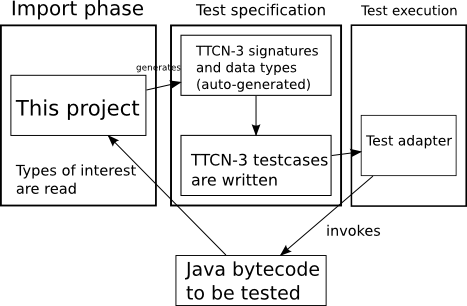
\includegraphics{workflow}
\caption{Expected workflow\label{fig:workflow}}
\end{figure}

In order to design a solution for this problem,
a more detailed specification of the requirements is needed.
The most important ones are listed below.
\begin{itemize}
\item Method invocation
\item Access to method return values and handling of exceptions
\item Accessor signatures (setters and getters) for public fields
\item Persistence of objects between calls
\item Predictable, stable auto-generated type names (detailed later)
\item Type safety (e.g.\ for method arguments)
\end{itemize}

The list starts with the functionality needed in order to write unit tests
and then includes some requirements
for productivity and usability by the test developers.

Indeed, the first objective is to provide test developers
with a mechanism to invoke methods,
examine the return value and handle exceptions.
This leads to the need of storing objects between calls
so that they may keep their state.
In addition to methods, constructors need to be called as well.
A unit test written in Java is able to read public fields
from the objects under test
(and also modify them if the fields are not \verb=final=).
The solution needs to offer this functionality as well
(as a consequence this will allow test developers
to access enumeration constants
since in Java these are {\tt public static final} fields of the class).

Objects are stateful so a mechanism for storing them must be provided.
Some type safety
(e.g.\ when passing arguments to \ac{TTCN-3} signatures
corresponding to Java methods)
is also desirable as it improves productivity and prevents mistakes
by reporting type errors at compile time.

The solution should generate \ac{TTCN-3} types corresponding to the Java ones.
The generated names should be predictable (if the Java names are known)
and stable i.e.\ they should not change if the Java class is modified
(e.g.\ by adding methods which overload existing ones).
An important issue to tackle is
the lack of support for overloaded signatures in \ac{TTCN-3}.

Other mappings defined for similar situations
(e.g.\ for \ac{CORBA} as defined in
\citep[sec.~4.3.2.6]{website:java2idl-mapping})
use the approach that non-overloaded methods keep their original name
and overloaded ones get their names mangled (using certain criteria).
That approach has the benefit of generating short names wherever possible
and using long, cumbersome names only where needed
(for methods with several overloads).

The target for this project is
to always generate the same mangled name for a particular method.
This will allow it to be used for testing software which is in development
(and subject to changes which may introduce overloads).
A stable naming scheme will not change generated names over time
and thus will not require test case modifications from the test developers.
